%# -*- coding: utf-8-unix -*-
%%==================================================
%% chapter01.tex for SJTU Master Thesis
%%==================================================

%\bibliographystyle{sjtu2}%[此处用于每章都生产参考文献]
\chapter{系统实现}
\label{chap:sys_implement}

上一章介绍了qscache系统的设计,这一章将首先介绍qscache系统实现所需的预备知识,进而介绍qscache系统的具体实现。

\section{预备知识}

由于qscache系统位于linux内核态,因此需要对内核中与系统实现相关的基本知识进行介绍。这些预备知识包括Linux存储层次、bio、Device Mapper等。

\subsection{Linux存储层次}

Linux存储层次如图\ref{fig:linux_storage_layer}所示,大致可分为共六层\cite{敖青云2011存储技术原理分析}:

\begin{enumerate}
    \item 最上层位于用户态,对用户看到的文件,用户的应用程序通过调用POSIX接口对这些文件进行操作。

    \item 第二层为虚拟文件系统(VFS, virtual file system)层,位于内核态。VFS的作用为屏蔽其所管理的具体文件系统,使用户可以使用统一的接口进行调用。POSIX在VFS层将数据封装成bio,然后将bio交给挂载的具体文件系统执行操作,bio将在\ref{sec:bio}具体介绍。

    \item 第三层为块层(block layer),位于内核态。块层负责将bio封装成设备请求(request)。具体封装方法为:如果几个bio的读写区域连续,那么将他们积攒成一个request,request下挂多个连续bio,即合并bio请求。如果bio跟其它bio都不连续,则它自己创建一个新request,将自己挂到这个request下。每个request下能挂的bio有限,多个连续bio的访问总区域超过一定限额,就不能合并为一个request。之所以不将多个bio合并为一个bio而是使用request,是因为每个bio都有自己的回调,如果合并为一个bio则失去了对不同bio使用不同回调的灵活性。合并后的request会以队列的形式组织起来,等待SCSI层进行处理。

    \item 第四层为SCSI层,位于内核态。SCSI层负责将request封装成与块设备具体存储格式相关的SCSI命令。

    \item 第五层为设备驱动(device driver)层,位于内核态,负责接收SCSI命令,并将其转换为设备请求,将其放入设备请求队列。

    \item 第六层为具体的设备层,位于内核态,负责接收设备请求,并在实际设备上执行对应的操作。

\end{enumerate}

\begin{figure}[!htbp]
    \centering
    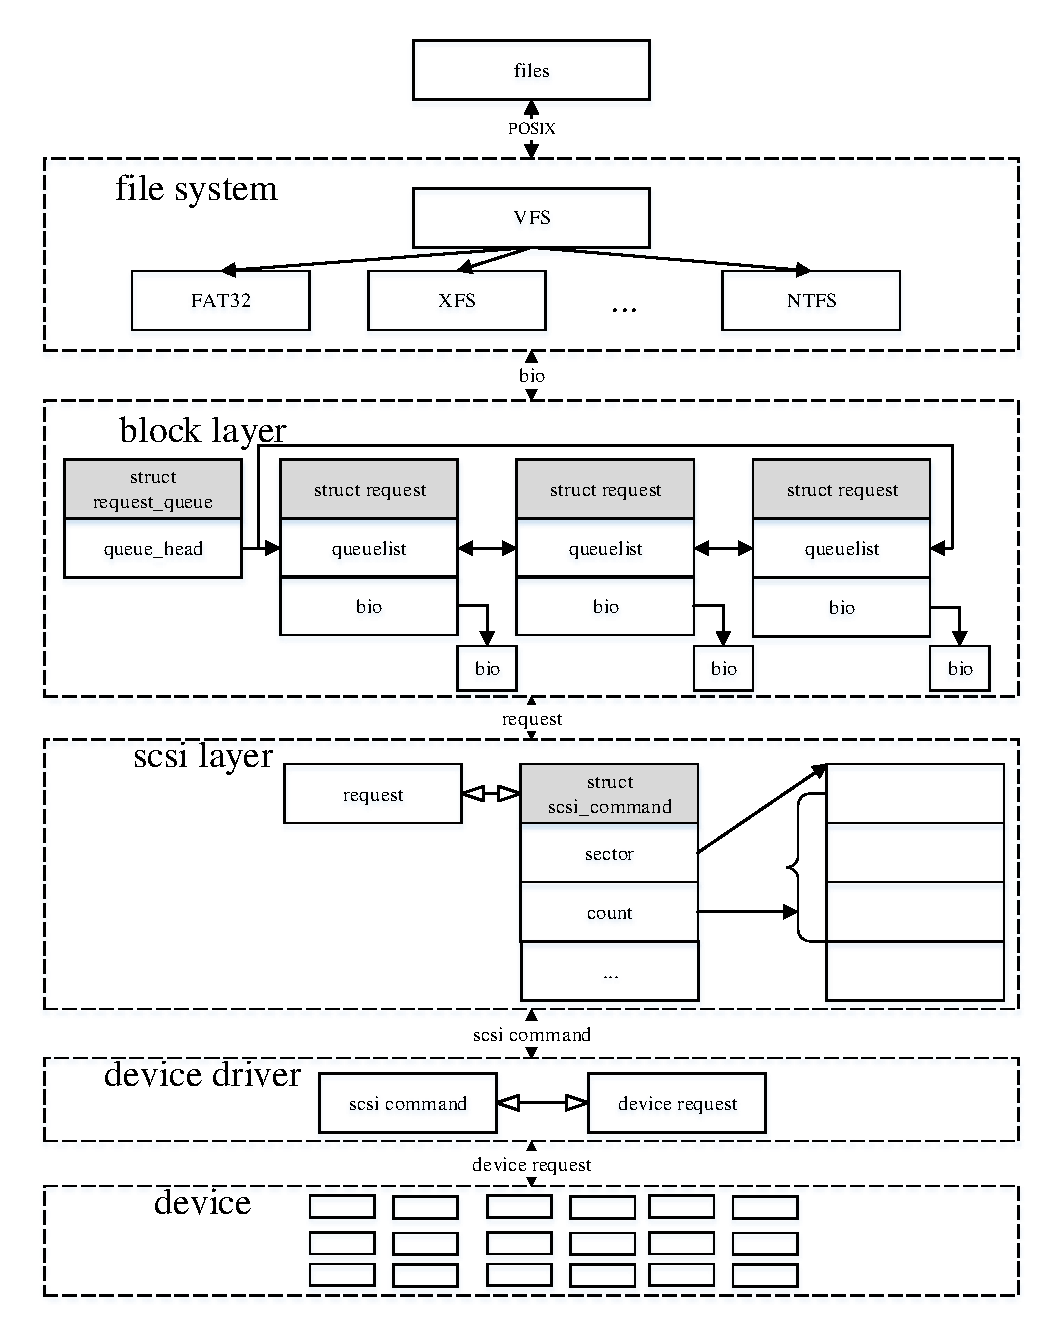
\includegraphics[width=\textwidth]{linux_storage_layer.pdf}
    \bicaption[fig:linux_storage_layer]{Linux存储层次}{Linux存储层次}{Fig.}{linux storage layer}
\end{figure}

\subsection{bio}
\label{sec:bio}

bio这一数据结构被用来描述块设备的I/O操作,将内存缓冲区与块设备联系起来的重要桥梁\cite{corbet2005linux}。

bio的具体结构如图\ref{fig:bio}所示。一个bio指针指向由bio结构体组成的链表,bio结构体中的bi\_io\_vec指向一个bi\_vec结构体数组,每个bi\_vec结构体中bv\_page指向内存中的实际页,bv\_offset和bv\_len组合来定位数据在该页中的具体位置,如此,一个bio链表就将散落在内存中的各数据组织为一个块设备请求。

\begin{figure}[!htbp]
    \centering
    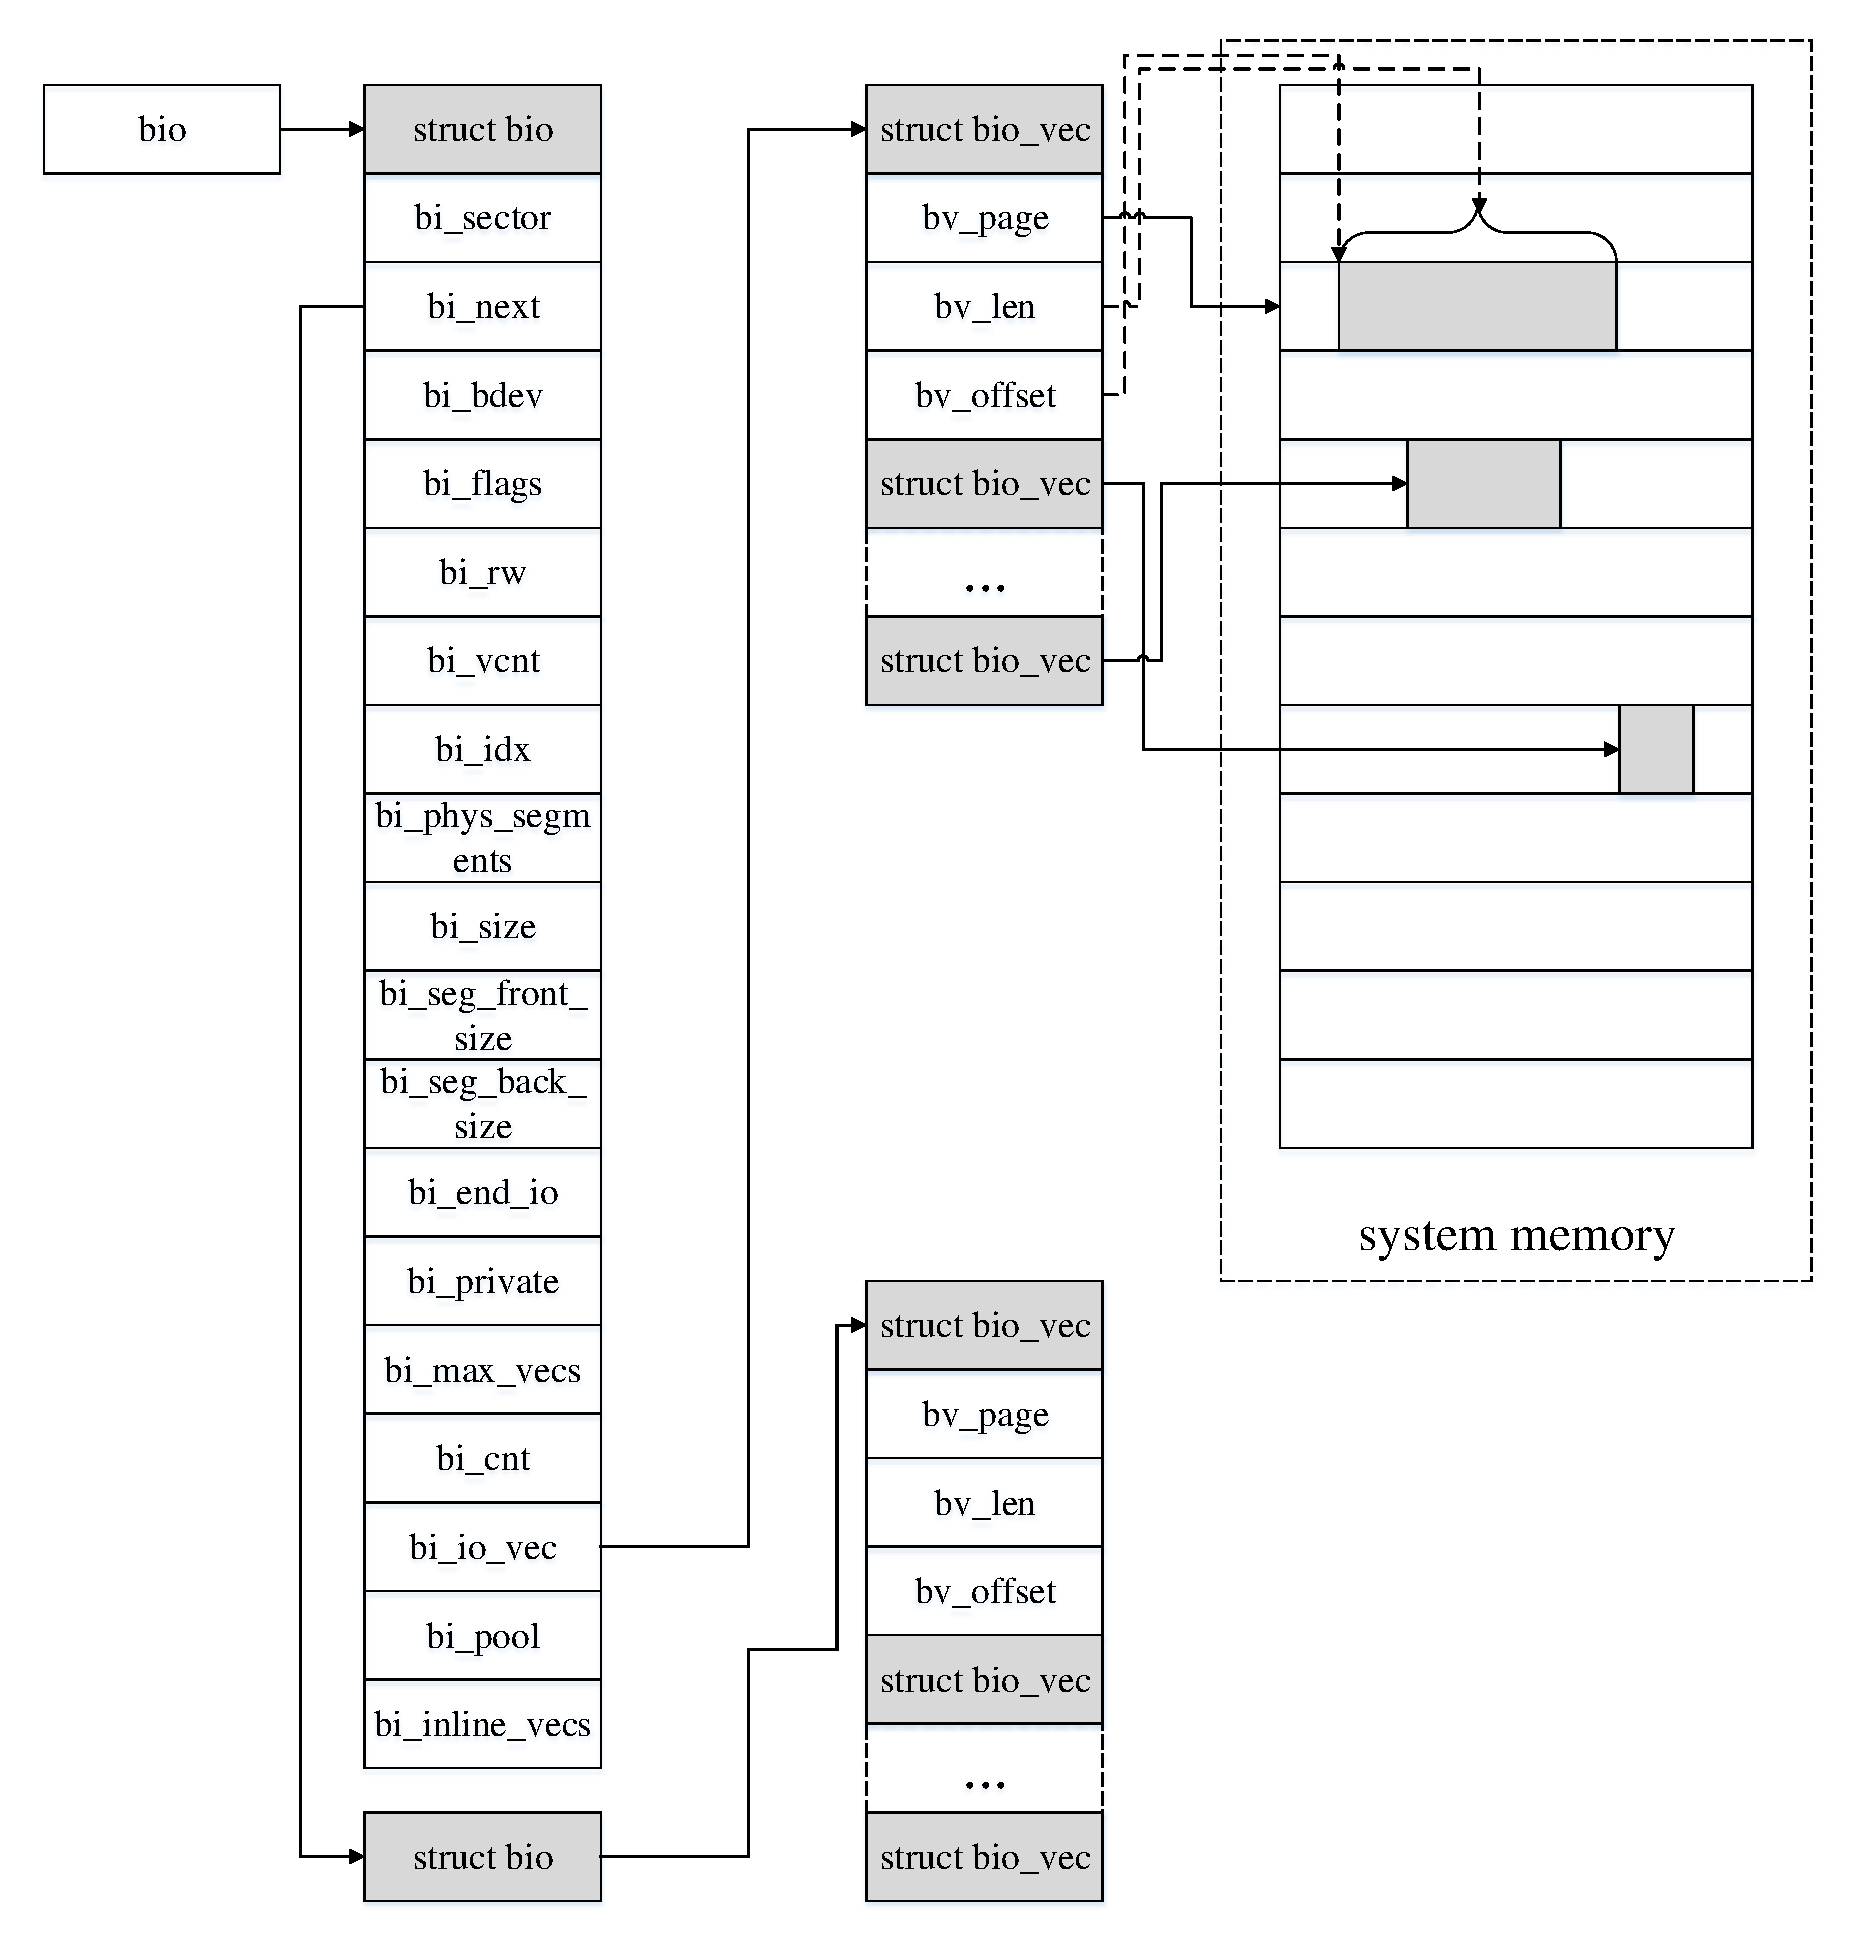
\includegraphics[width=0.8\textwidth]{bio.pdf}
    \bicaption[fig:bio]{bio结构}{bio结构}{Fig.}{bio structure}
\end{figure}

\subsection{Device Mapper}

Device Mapper是Linux2.6 内核中支持逻辑卷管理的通用设备映射机制,它为实现用于存储资源管理的块设备驱动提供了一个高度模块化的内核架构\cite{bovet2005understanding}。Device Mapper以一个块设备驱动在内核中注册,它包含mapped device、mapping table、target device这三个重要概念。mapped device可以理解为内核对外提供的逻辑设备,用户看到的也是这个逻辑设备,mapped device通过mapping table组织与与target device的映射关系,一个mapped device可以映射到一个或者多个target device上,总体层次如图\ref{fig:device_mapper}所示,target device可以是真实的物理设备也可以是另一个mapped device,如此迭代,形成一个树状结构。

\begin{figure}[!htbp]
    \centering
    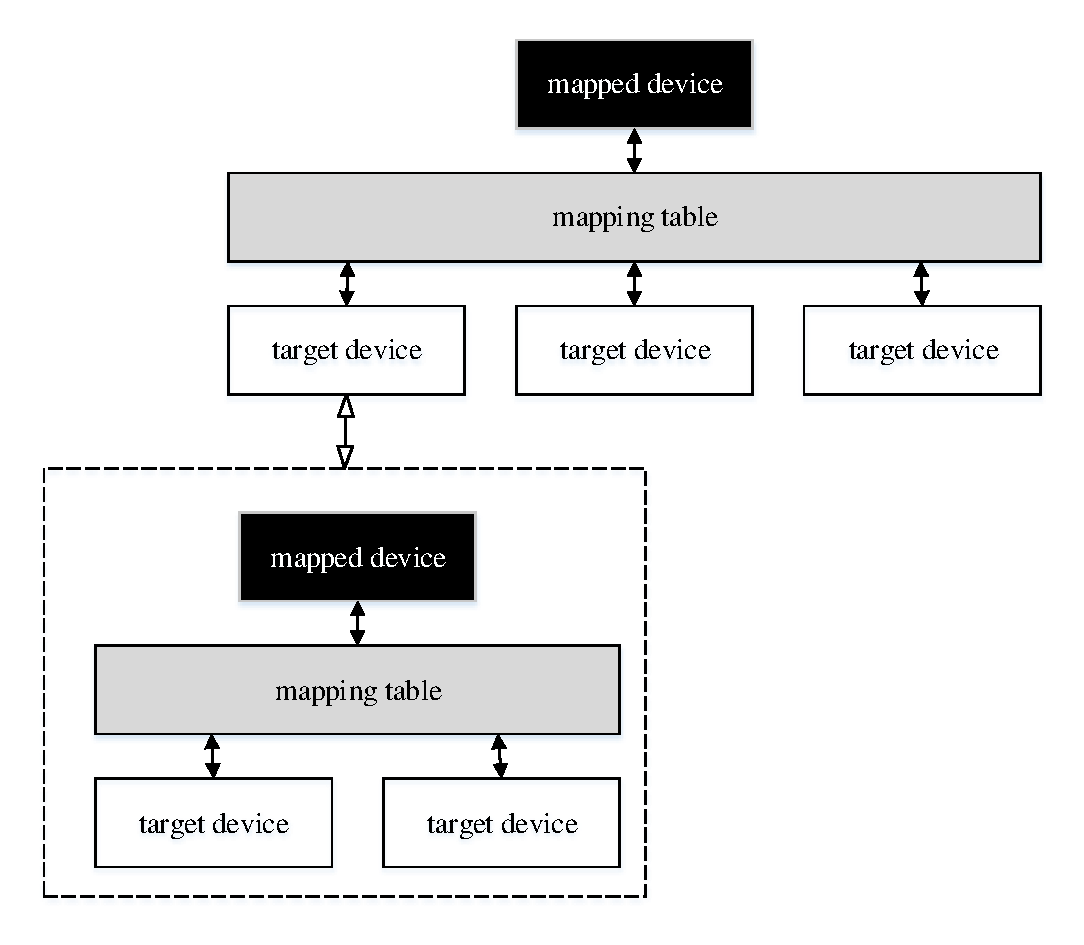
\includegraphics[width=0.8\textwidth]{device_mapper.pdf}
    \bicaption[fig:device_mapper]{Device Mapper层次图}{Device Mapper层次图}{Fig.}{Device Mapper Layer}
\end{figure}

Device Mapper的实现原理是将mapped device的make\_request\_fn方法实现为自己的dm\_request,这个经过mapped device的bio请求都会进入dm\_request方法,之后Device Mapper通过判断mapped device是基于request还是基于bio来分别处理:

如果mapped device是基于request的,那么和磁盘设备一样通过generic\_make\_request把bio合并为request,将其放到mapped device的request队列中,当mapped device通过kblockd调用dm\_request\_fn时,dm\_request\_fn中会调用peek\_request从mapped device的request队列中拿出request将其clone(clone生成的request中的bio与原request中的bio指向同一个内存页,clone操作只是分配新的bio和request),然后通过调用map\_request将request映射,将clone后的request发往低层的真实设备。

如果mapped device是基于bio的,那么调用\_dm\_request首先clone bio然后调用\_\_map\_bio将bio映射,将clone后的bio通过generic\_make\_request发往低层的真实设备。

mapped device基于request还是基于bio的主要区别在于,如果是基于request则request是放在mapped device的request队列中,如果是基于bio,则是在调用generic\_make\_request总将bio封装成request放到真实设备的request队列中。


\subsection{其他预备知识}

在qscache系统的实现过程中,除了上面介绍的几个关键知识点外,还涉及很多其他的Linux内核知识,比如Linux的内核模块编程、内核编程中的常用宏、常用数据结构、内核的调试等内容,这里不再详细介绍。

\section{编程实现}

有了上面预备知识的铺垫,就可以比较清楚地介绍qscache系统的编程实现了。下面将着重介绍qscache系统基于Device Mapper机制的系统架构实现、系统信息组织与管理的实现、冷热数据识别算法的实现以及多缓存设备对多后台设备的实现。本系统基于的内核版本为linux 3.10.108。

\subsection{系统架构实现}

qscache系统基于Linux的Device Mapper实现,通过研究Linux内核中Device Mapper的相关代码,本研究发现Device Mapper中使用target\_type这一结构体用来管理对mapped device的各种操作,target\_type的主要成员类型及作用见表\ref{tab:target_type}。因此需要定义qscache对应的target\_type,使qscache系统可以通过Device Mapper组织管理不同设备。

\begin{table}[H]
    \centering
    \bicaption[tab:target_type]{target\_type的主要成员类型及作用}{target\_type的主要成员类型及作用}{Table}{structure of target\_type}
    \begin{tabular}{ccc} 
        \toprule
        成员 & 类型 & 作用\\
        \midrule
        name & const char* & Device Mapper模块的名字 \\ 
        module & struct module* & 对应的Device Mapper模块 \\ 
        version & unsigned[3] & 版本号 \\ 
        ctr & dm\_ctr\_fn & 设备的构造函数 \\ 
        dtr & dm\_dtr\_fn & 设备的析构函数 \\ 
        map & dm\_map\_fn & 指向负责将bio请求重映射的函数 \\ 
        map\_rq & dm\_map\_request\_fn & 指向负责将request请求重映射的函数 \\ 
        end\_io & dm\_endio\_fn & 指向当bio结束时调用的函数 \\ 
        rq\_end\_io & dm\_request\_endio\_fn & 指向当request结束时调用的函数 \\ 
        status & dm\_status\_fn & 指向返回设备状态的函数 \\ 
        message & dm\_message\_fn & 指向负责处理发送给设备的命令的函数 \\ 
        ioctl & dm\_ioctl\_fn & 指向负责处理通过ioctl对设备管理的函数 \\ 
        iterate\_devices & dm\_iterate\_devices\_fn & 指向负责遍历处理与设备相关的设备的函数 \\ 
        \bottomrule
    \end{tabular}
\end{table}

另外qscache系统对于I/O带宽按权限进行分配的功能将通过使用Linux自带的I/O调度器的CFQ策略,通过为不同进程设置不同的cgroup的weight实现对这些进程按照权重不同分配不同的I/O带宽,但是由于I/O调度器只对request队列起作用,对bio不起作用,因此qscache系统将实现基于bio模式启动与基于request模式启动,对于不同的模式分别定义不同的target\_type然后在模块加载时注册不同的target\_type就以不同模式启动了。但是本研究发现现有的Device Mapper提供的target\_type并不能很好地实现基于request的模式,因此下面将分别对基于bio模式与基于request模式的公用接口函数的实现、基于bio模式的实现以及基于request模式的实现展开详细介绍。

\subsubsection{公用接口函数的实现}

qscache系统的公用接口函数为ctr、dtr、status、ioctl、iterate\_devices这五个,下面将分别进行介绍。

ctr接口的实现流程如图\ref{fig:qscache_ctr}所示,ctr负责接收用户传来的各种参数,对相关结构体进行内存的申请工作,对相关的工作队列、等待队列等进行初始化操作,以及对相关参数进行设置,当操作出错时释放已申请的内存空间并返回。

\begin{figure}[H]
    \centering
    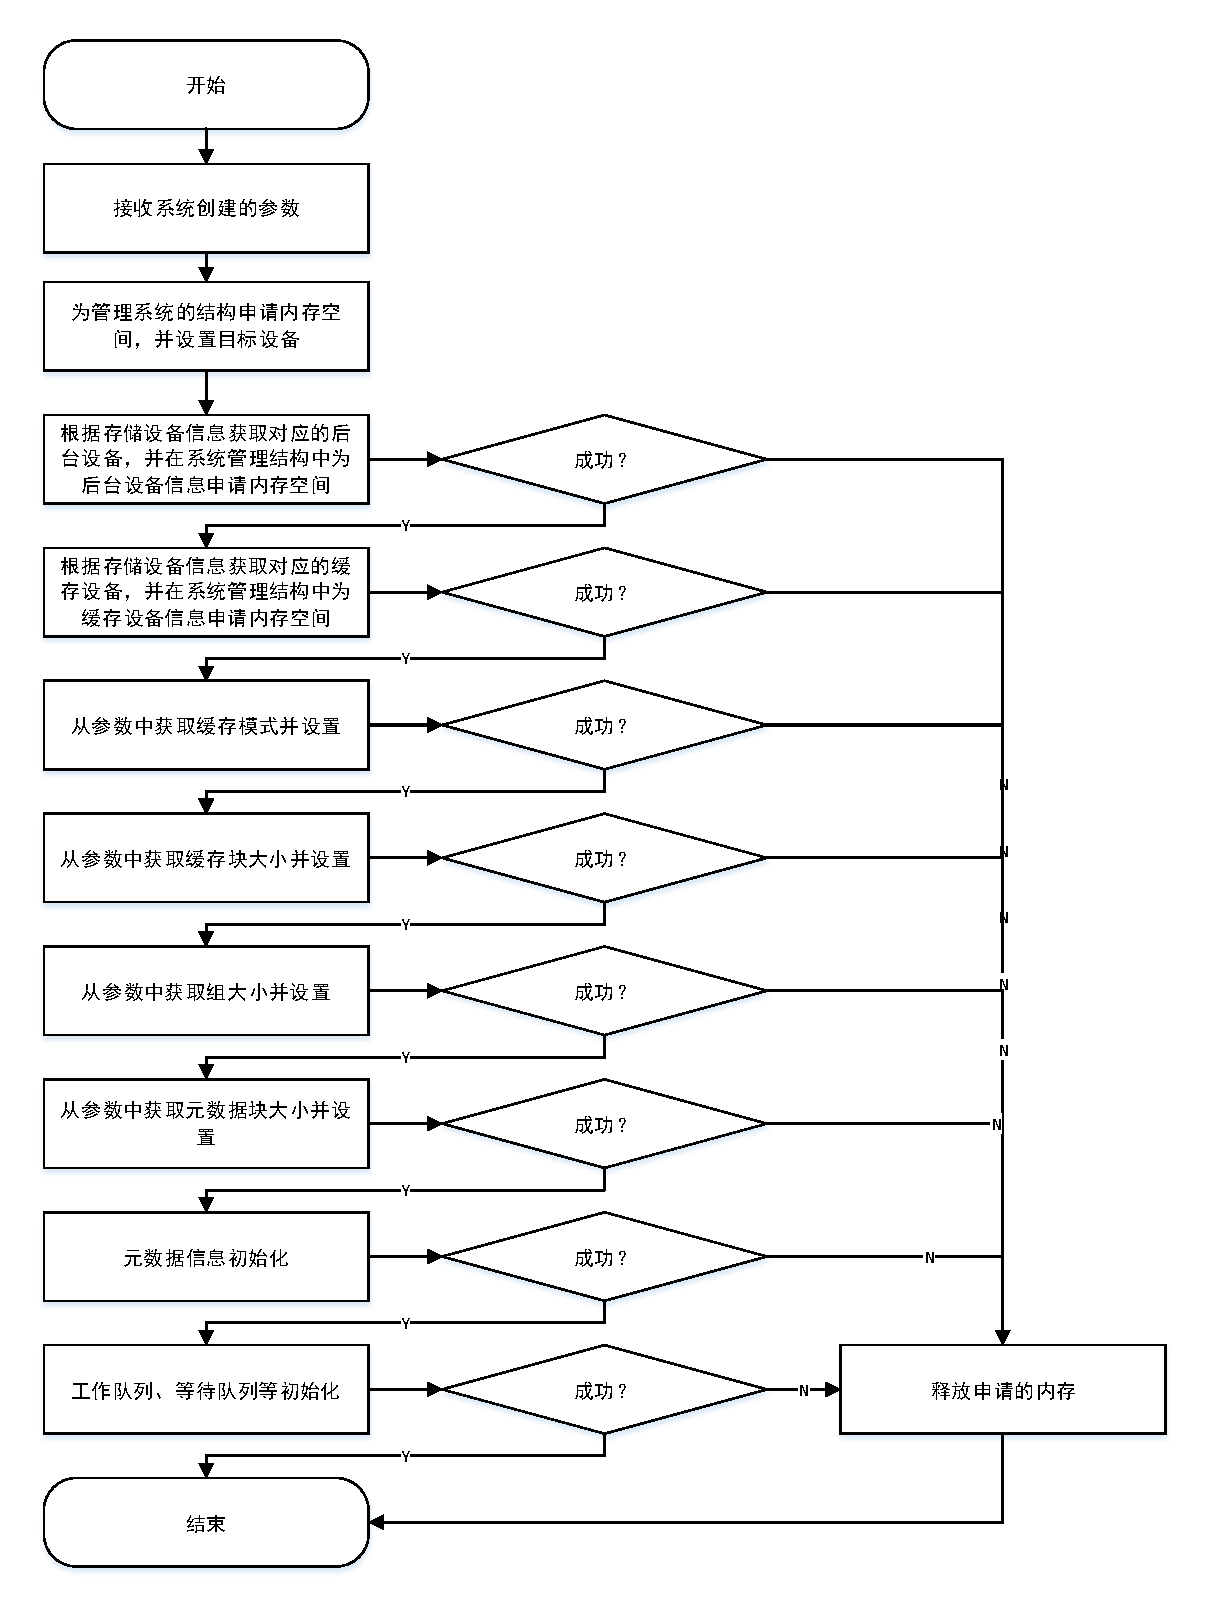
\includegraphics[width=0.8\textwidth]{qscache_ctr.pdf}
    \bicaption[fig:qscache_ctr]{qscache的ctr接口}{qscache的ctr接口}{Fig.}{process of qscache ctr}
\end{figure}

dtr接口的实现比较简单,就是将在ctr接口中申请的各种资源依倒序依次释放,保证系统占用的资源都返还操作系统,不会发生内存泄露的情况。

status接口负责根据系统记录的信息返回系统的当前状态供用户查询,通过status接口,用户可以得到读命中次数、写命中次数、脏数据命中次数、缓存块替换次数、对缓存设备的读写次数、对后台设备的读写次数、缓存设备的容量使用情况、后台设备的容量使用情况、未缓存的操作数等信息。

ioctl接口负责处理通过ioctl对设备的管理操作,主要接收用户传来的参数对系统的进程黑名单和进程白名单进行增删操作。

iterate\_devices接口负责遍历系统所管理的缓存设备和后台设备,对它们调用指定的函数。

\subsubsection{基于bio模式的实现}

基于bio模式的实现主要是target\_type中map接口的实现,map是整个系统数据的入口,map负责对bio请求进行解析,并根据请求的操作类型分别交由不同函数处理。

对于读请求的处理如图\ref{fig:qscache_map_read}所示。首先判断请求是否为可以被缓存的请求,判断的依据是判断进程是否在黑名单中以及依据参数的设置决定是否要缓存顺序请求,如果不能被缓存则直接提交到后台设备执行读操作,如果可以被缓存,则首先在缓存设备中查找数据块,如果找到对应数据块,则将请求提交到缓存上执行读操作,如果没有找到数据块,则将请求提交到后台设备上执行读操作,并根据操作是否可以被缓存以及数据块的热度决定是否要替换缓存块执行对应的缓存块操作。

\begin{figure}[H]
    \centering
    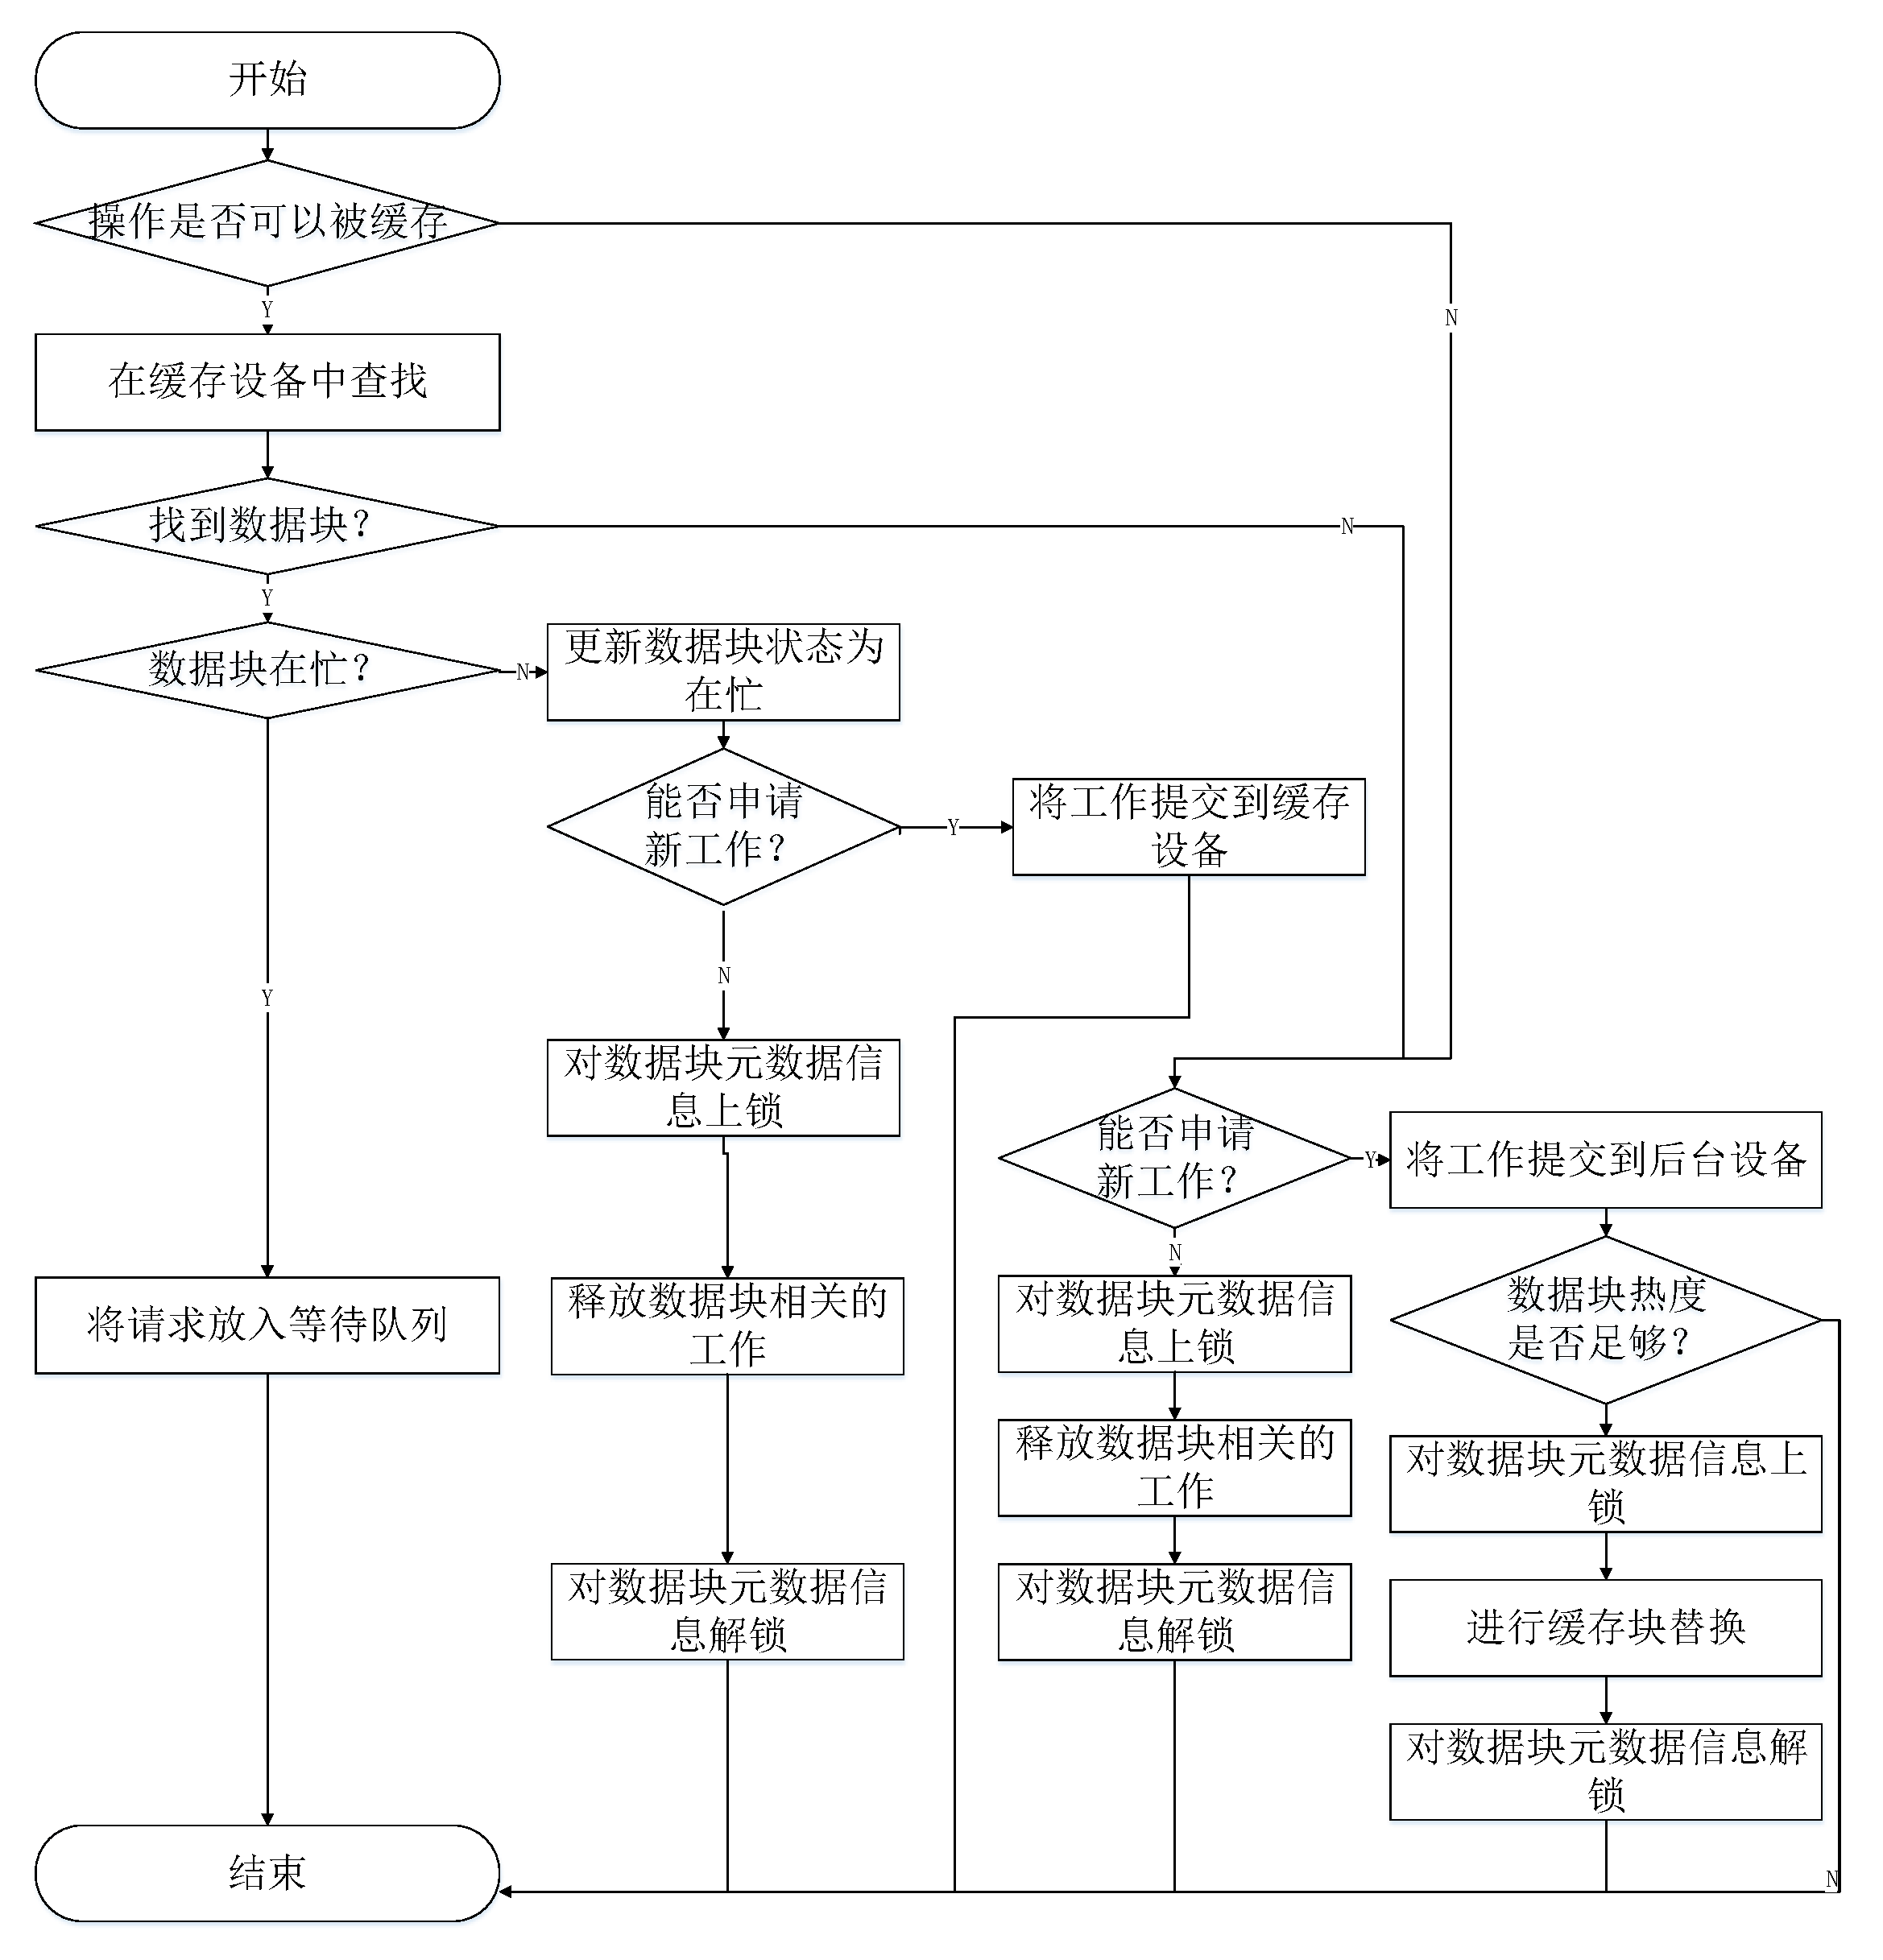
\includegraphics[width=0.8\textwidth]{qscache_map_read.pdf}
    \bicaption[fig:qscache_map_read]{qscache的map接口读请求处理}{qscache的map接口读请求处理}{Fig.}{process of qscache map read}
\end{figure}

对于写请求的处理如图\ref{fig:qscache_map_write}所示。首先判断请求是否为可以被缓存的请求,判断的依据是判断进程是否在黑名单中以及依据参数的设置决定是否要缓存顺序请求,如果不能被缓存则直接提交到后台设备执行写操作,如果可以被缓存,则首先在缓存设备中查找数据块,如果找到对应数据块,则将请求提交到缓存上执行写操作,并判断是否为写穿模式,如果为写穿模式则也将请求提交到后台设备上执行写操作,如果没有找到数据块,则将请求提交到后台设备上执行写操作,并根据操作是否可以被缓存以及数据块的热度决定是否要替换缓存块执行对应的缓存块操作。

\begin{figure}[H]
    \centering
    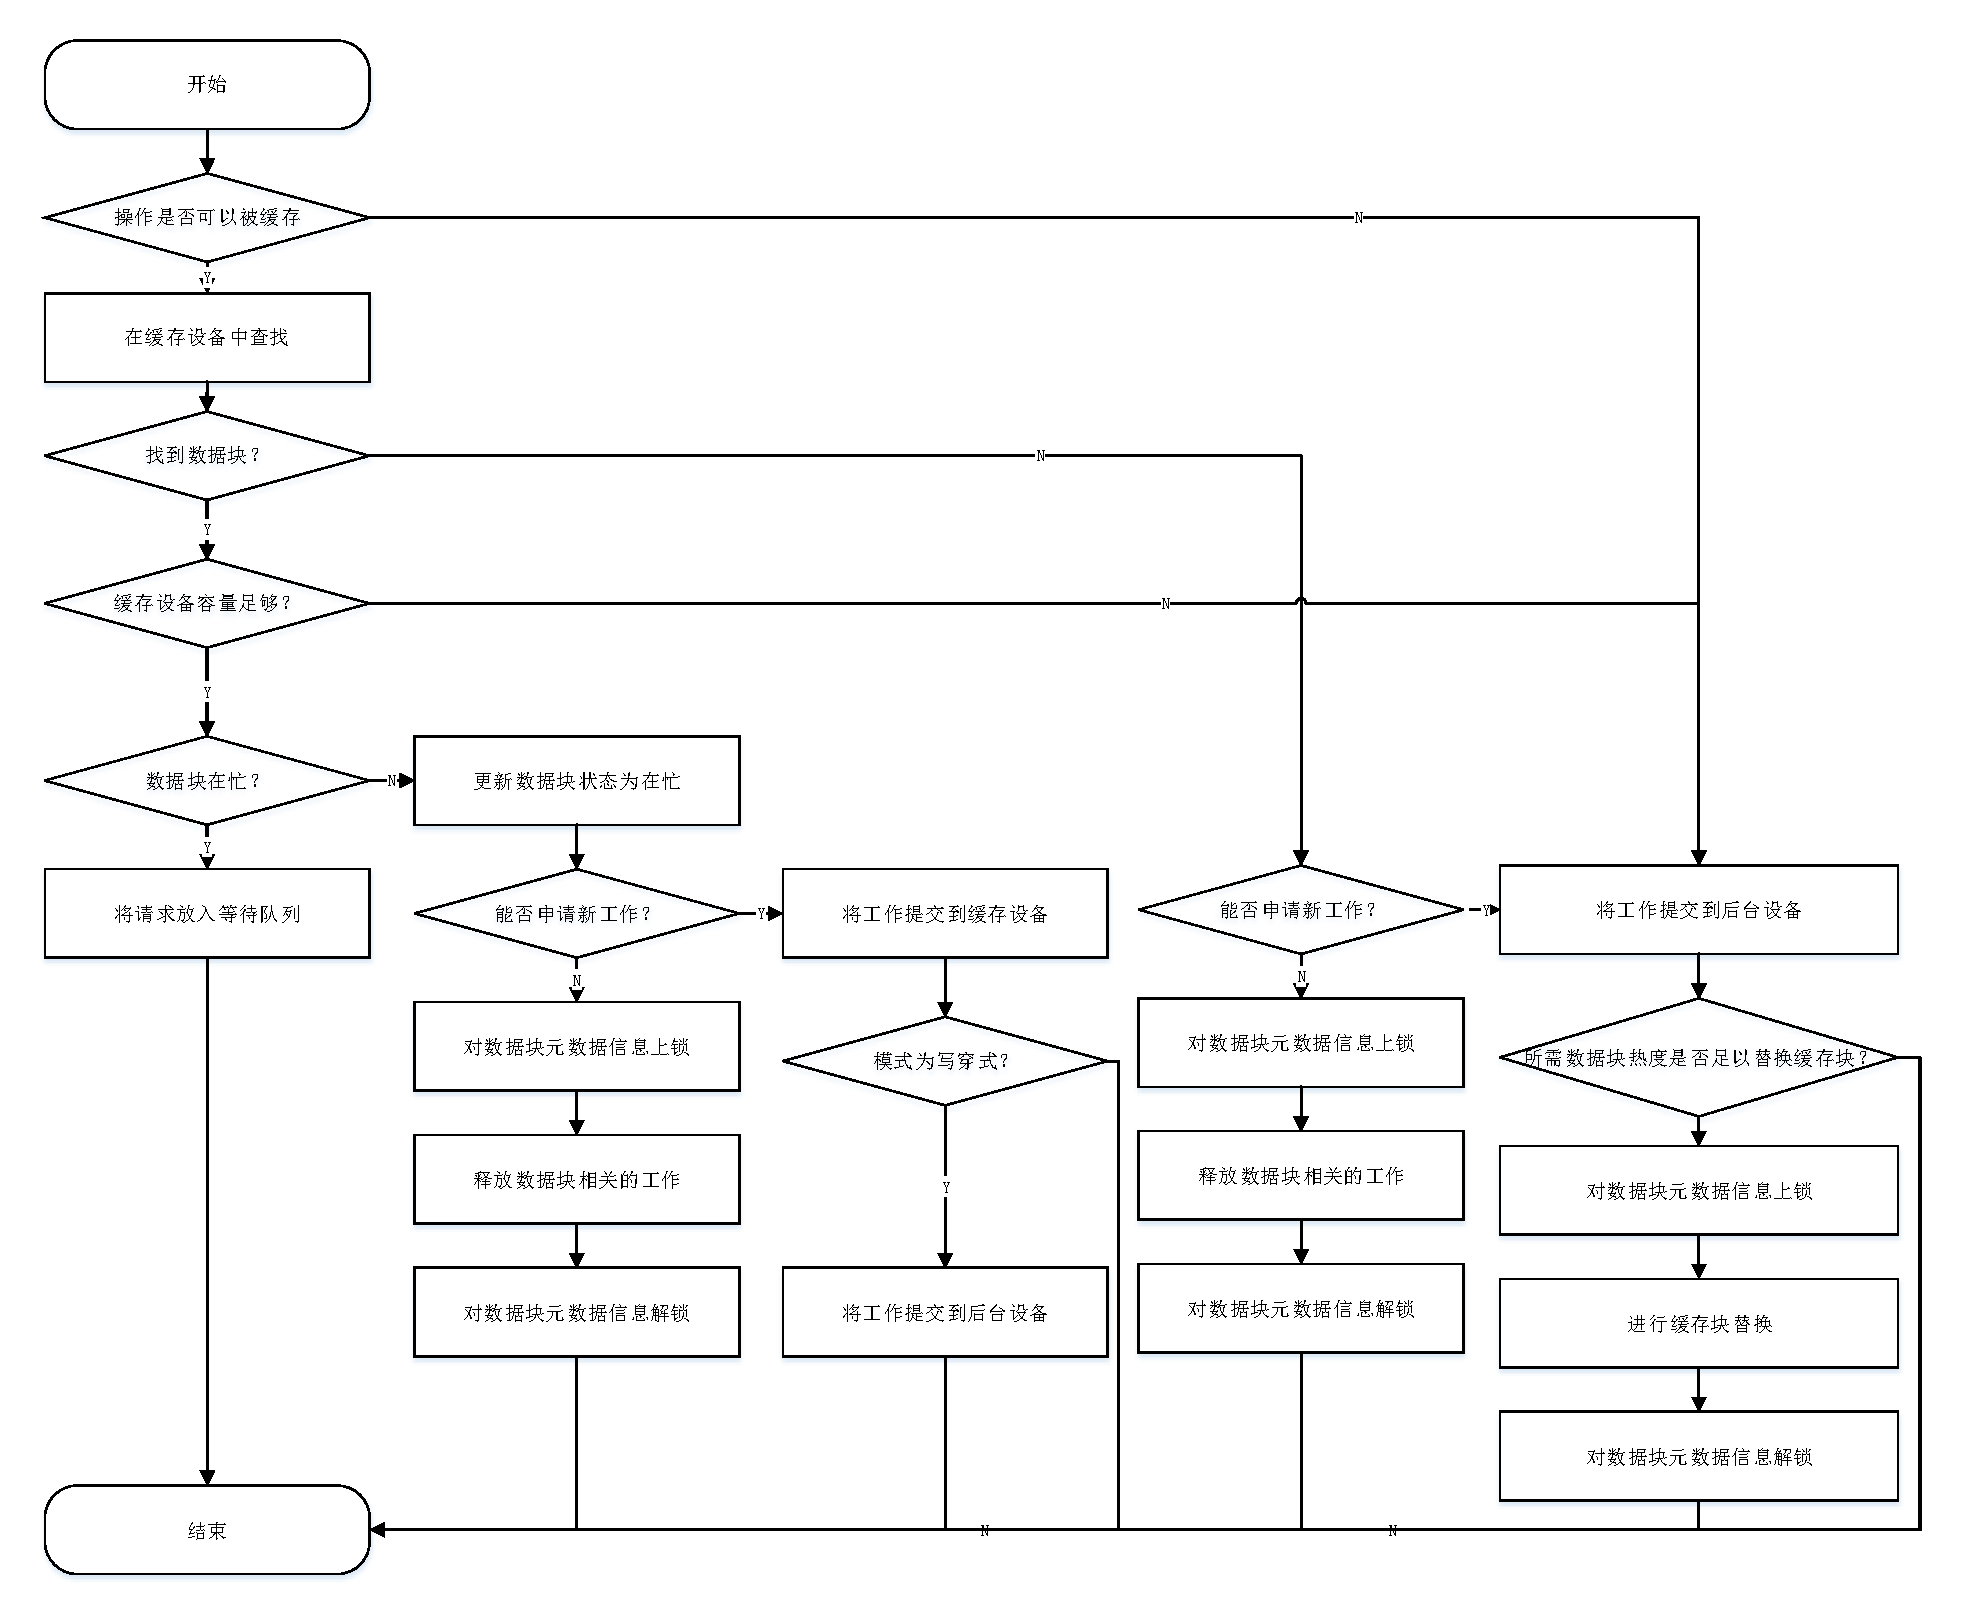
\includegraphics[width=0.8\textwidth]{qscache_map_write.pdf}
    \bicaption[fig:qscache_map_write]{qscache的map接口写请求处理}{qscache的map接口写请求处理}{Fig.}{process of qscache map write}
\end{figure}

\subsubsection{基于request模式的实现}

本研究发现现有的Device Mapper的实现中,仅有multipath\_target是基于request的target\_type,而在multipath\_target中map\_rq的实现multipath\_map仅仅是改变request队列然后返回DM\_MAPIO\_REMAPPED,而混合存储系统中map\_rq必须负责将对mapped device的请求映射到低层的设备因此不能仅仅像multipath\_target中map\_rq的实现一样简单。因此需要实现一个新的接口。在target\_type中添加make\_rq接口实现用bio生成request,然后依靠map\_rq将请求映射到不同的低层设备。

对Linux的内核作出的具体修改如下:

\begin{enumerate}
    \item include/linux/dm-io.h文件对dm\_io\_request结构体添加三个变量,submit\_bio用以表示是否直接提交bio,start和end为两个bio指针,指向该dm\_io\_request的起始bio和终止bio。
    \item drivers/md/dm-io.c文件,do\_region改为接收dm\_io\_request类型参数,依据dm\_io\_request类型的参数中submit\_bio的设置判断是直接提交bio还是放入request中。dispatch\_io改为接收dm\_io\_request类型参数,相关操作包括对do\_region的调用相应改为基于dm\_io\_request类型的操作。sync\_io改为接收dm\_io\_request类型参数,相关操作包括对dispatch\_io的调用相应改为基于dm\_io\_request类型的操作。async\_io改为接收dm\_io\_request类型参数,相关操作包括对dispatch\_io的调用相应改为基于dm\_io\_request类型的操作。dm\_io中对sync\_io和async\_io的调用都改为传递dm\_io\_request类型参数。
    \item include/linux/device-mapper.h文件中对target\_type结构体添加函数指针make\_rq作为新的新接口,用以支持自己对request的生成。
    \item drivers/md/dm.c文件,dm\_request原本只是简单地判断mapped device是基于request还是基于bio,并据此分别调用blk\_queue\_bio或\_dm\_request。现在首先从映射表中获得mapped device,查看是否实现了具体的make\_rq方法,如果实现了则调用该方法然后返回,否则依旧根据是基于request还是基于bio分别调用blk\_queue\_bio或\_dm\_request,流程如图\ref{fig:dm_request}所示。

    \begin{figure}[!htbp]
        \centering
        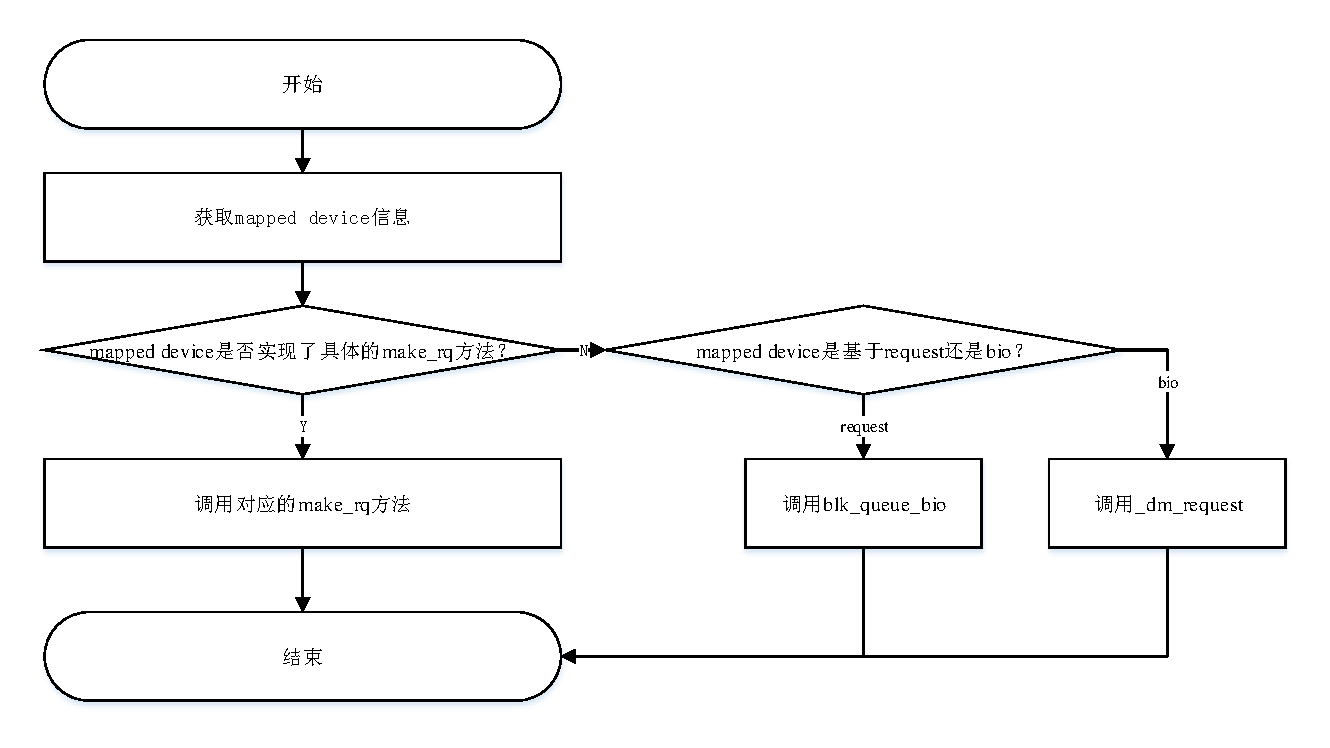
\includegraphics[width=\textwidth]{dm_request.pdf}
        \bicaption[fig:dm_request]{dm\_request处理流程}{dm\_request处理流程}{Fig.}{dm\_request process}
    \end{figure}

    \item drivers/md/dm-bufio.c文件,use\_dmio和dm\_bufio\_issue\_flush中初始化io\_req时设置submit\_bio为1,默认直接提交bio。
    \item drivers/md/dm-kcopyd.c文件,run\_io\_job中初始化io\_req时设置submit\_bio为1,默认直接提交bio。
    \item drivers/md/dm-log.c文件,create\_log\_context中设置lc的io\_req的submit\_bio为1,默认直接提交bio。
    \item drivers/md/dm-raid1.c文件,mirror\_flush、read\_async\_bio和do\_write中初始化io\_req时设置submit\_bio为1,默认直接提交bio。
    \item drivers/md/dm-snap-persistent.c文件,chunk\_io中初始化io\_req时设置submit\_bio为1,默认直接提交bio。
\end{enumerate}

在对Linux内核修改完毕后,现在的Device Mapper中target\_type支持开发者实现自己的make\_rq接口。qscache系统通过实现make\_rq和map\_rq接口实现基于request的混合存储系统,具体流程如图\ref{fig:request_process}所示。make\_rq()负责用bio生成对应的request而map\_rq()负责将对混合存储系统的请求分派到具体的实际设备执行操作。

\begin{figure}[!htbp]
    \centering
    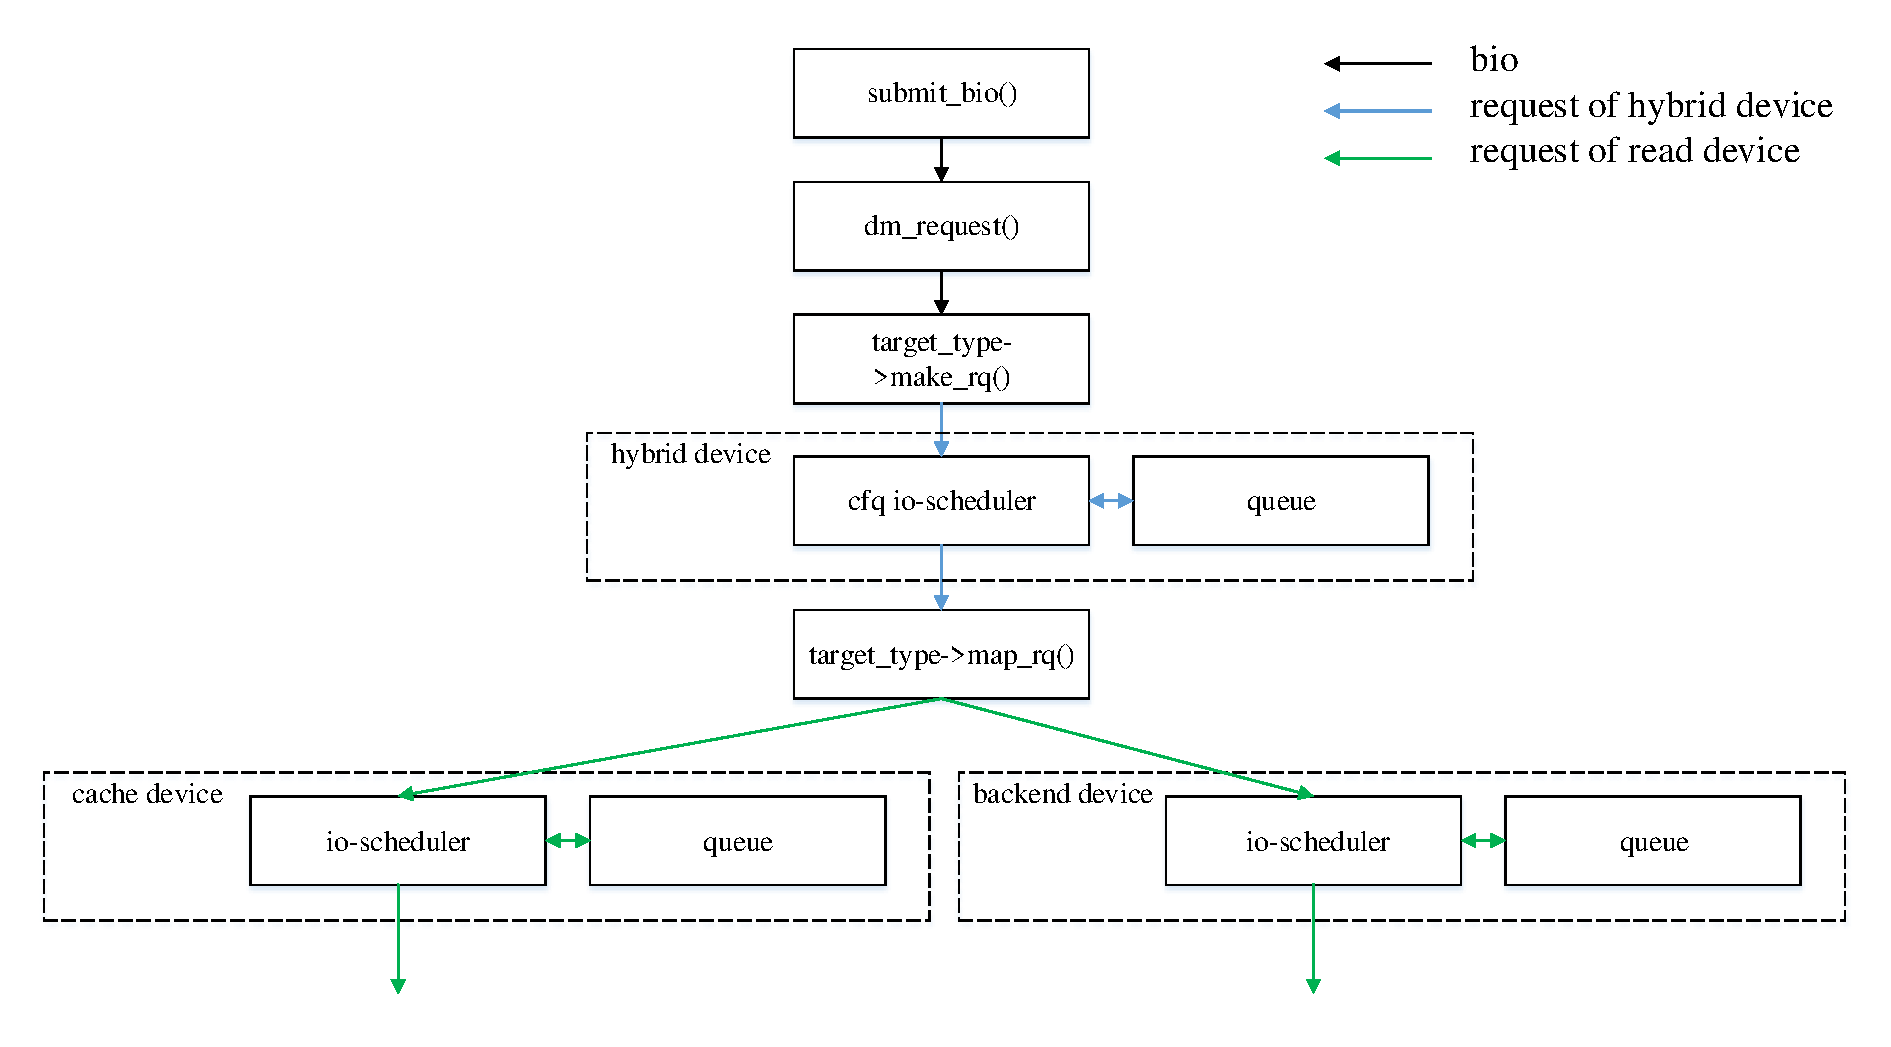
\includegraphics[width=0.9\textwidth]{request_process.pdf}

    \vskip -1cm

    \bicaption[fig:request_process]{基于request的请求流程}{基于request的请求流程}{Fig.}{request process in request-based system}
\end{figure}

具体地说,make\_rq()接收对系统的bio请求,然后根据bio判断对系统的具体操作,然后去调用对应操作的函数并传入参数设置不立即提交bio,各操作函数经过递归调用最后都会落到dm\_io\_async\_bvec()中,如图\ref{fig:dm_io_async_bvec}所示,make\_rq()不论是调用不经缓存的操作,还是缓存命中或未命中的读写操作最终都会调用dm\_io\_async\_bvec(),并在make\_rq()中将是否立即提交bio的参数一路传给dm\_io\_async\_bvec()。

\begin{figure}[H]
    \centering
    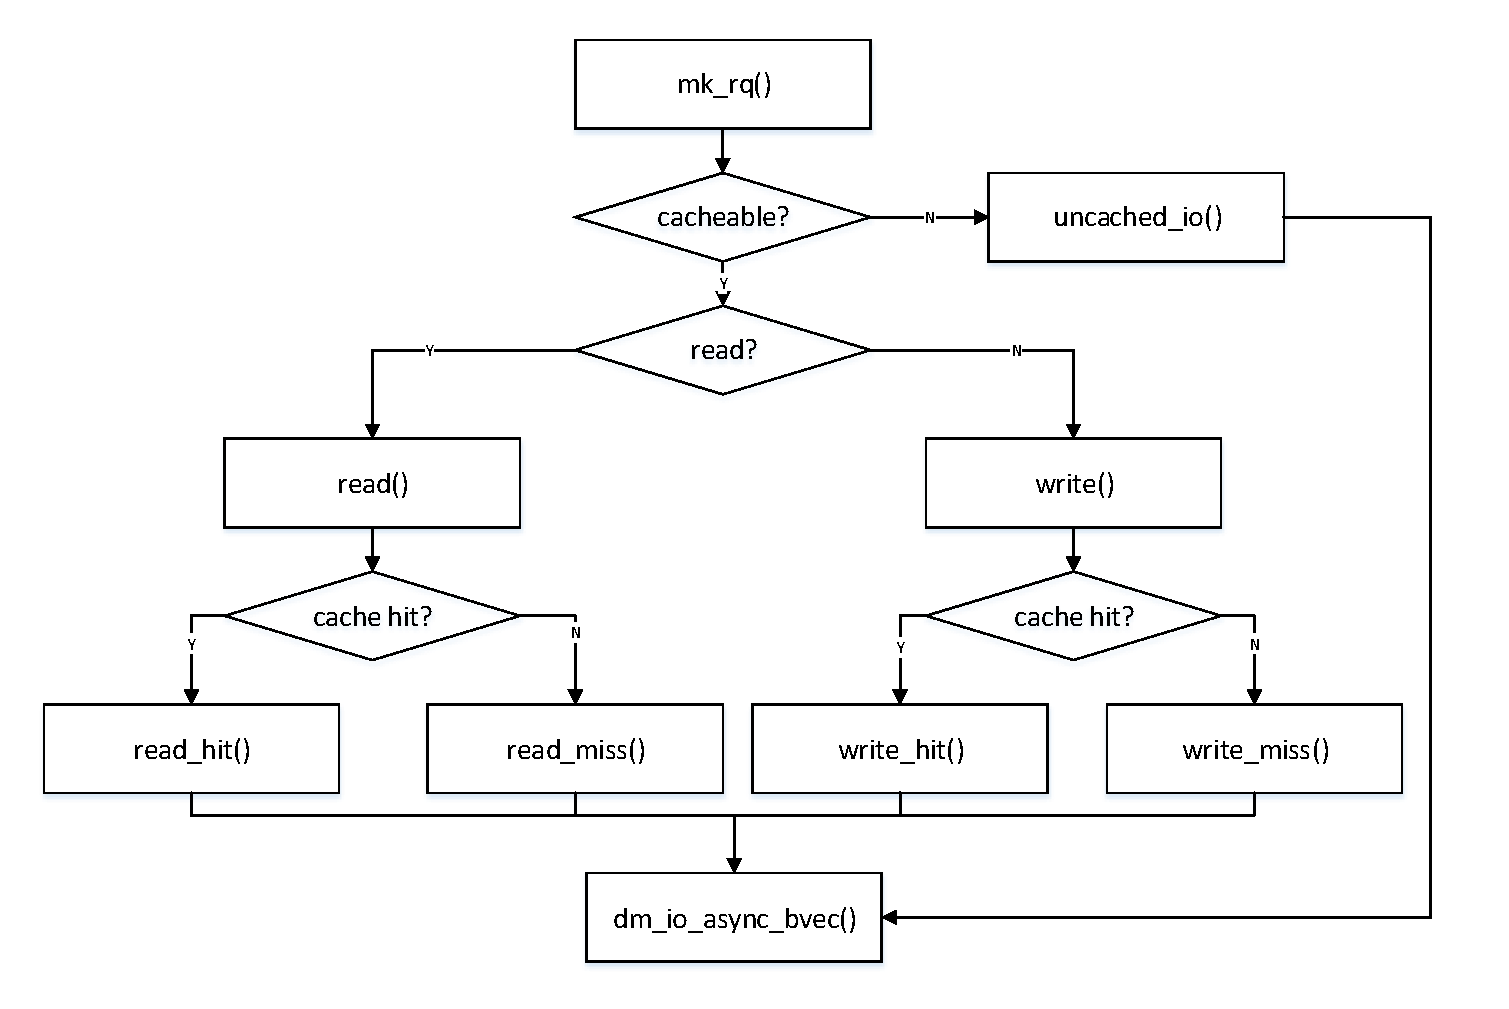
\includegraphics[width=\textwidth]{call_dm_io_async_bvec.pdf}
    \bicaption[fig:call_dm_io_async_bvec]{dm\_io\_async\_bvec()调用流程}{dm\_io\_async\_bvec()调用流程}{Fig.}{call of dm\_io\_async\_bvec()}
\end{figure}

dm\_io\_async\_bvec()的处理流程如图\ref{fig:process_dm_io_async_bvec}所示,dm\_io\_async\_bvec()根据传入的参数生成dm\_io\_request并调用dm\_io(),对于立即提交的bio,dm\_io\_async\_bvec()结束调用后就立刻返回,对于不是立即提交的bio,再dm\_io()中会设置整个bio的开始与结束,然后返回dm\_io\_async\_bvec()通过开始与结束遍历这些bio,然后用这些bio各自或生成一个request放入队列中。

\begin{figure}[H]
    \centering
    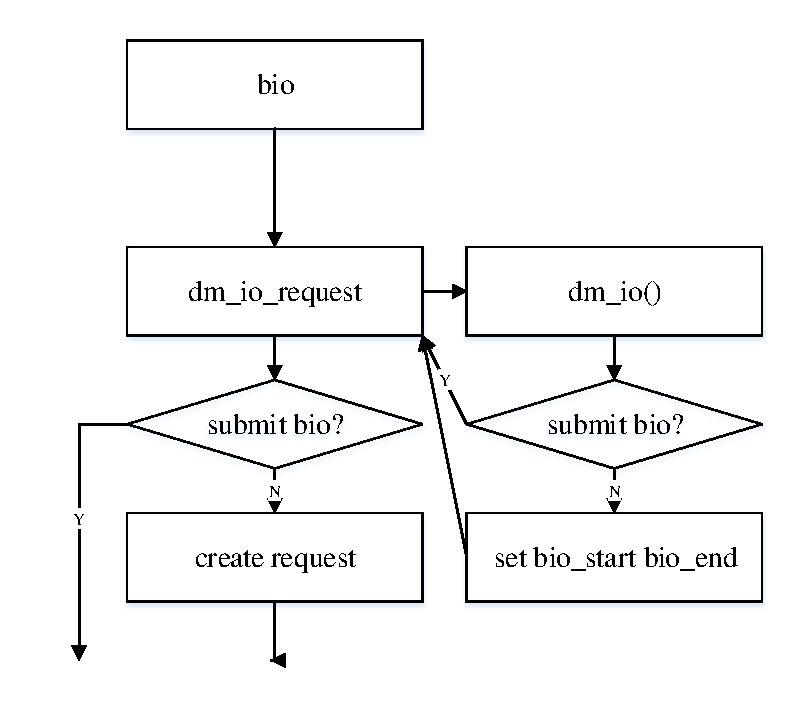
\includegraphics[width=\textwidth]{process_dm_io_async_bvec.pdf}
    \bicaption[fig:process_dm_io_async_bvec]{dm\_io\_async\_bvec()处理流程}{dm\_io\_async\_bvec()处理流程}{Fig.}{process of dm\_io\_async\_bvec()}
\end{figure}

\subsection{系统信息组织与管理的实现}

qscache系统的系统信息由一个全局的数据结构cache\_c进行统一管理。cache\_c中的主要成员类型及其作用如表\ref{tab:cache_c}所示。其他诸如黑名单、白名单也在cache\_c中。相关冷热数据识别要用到的数据结构,则以set为单位存放在cache\_sets这一结构体中。

\begin{table}[!htbp]
    \centering
    \bicaption[tab:cache_c]{cache\_c的主要成员类型及作用}{cache\_c的主要成员类型及作用}{Table}{structure of cache\_c}
    \begin{tabular}{ccc} 
        \toprule
        成员 & 类型 & 作用\\
        \midrule
        tgt & struct dm\_target* & Device Mapper中对target\_type的一层封装 \\ 
        disk\_dev & struct dm\_dev* & 管理与后台设备相关的信息 \\ 
        cache\_dev & struct dm\_dev* & 管理与缓存设备相关的信息 \\ 
        cache & struct cacheblock* & 管理缓存块的哈希表 \\ 
        cache\_sets & struct cache\_set* & 用于管理set \\ 
        size & sector\_t & 缓存大小 \\ 
        assoc & unsigned int & 缓存设备的set大小 \\ 
        block\_size & unsigned int & 缓存块的大小 \\ 
        disk\_assoc & unsigned int & 后台设备的set大小 \\ 
        num\_sets & unsigned int & set的数目 \\ 
        cache\_mode & int & 缓存模式:写回、写穿等 \\ 
        dirty\_thresh\_set & int & 每个set开始写回脏数据的阈值 \\ 
        max\_clean\_ios\_set & int & 每个set写回脏数据的量的阈值 \\ 
        dm\_vdevname & char[DEV\_PATHLEN] & 虚拟出来的设备名 \\ 
        cache\_devname & char[DEV\_PATHLEN] & 缓存设备的UUID \\ 
        disk\_devname & char[DEV\_PATHLEN] & 后台设备的UUID \\ 
        bypass\_cache & int & 是否略过缓存 \\      
        \bottomrule
    \end{tabular}
\end{table}

\subsection{冷热数据识别算法的实现}

在qscache系统中采用双层LRU链表,具体思想见\ref{sec:data_hot_identification}。系统为每个set建立两个LRU链表,在管理cache的cache\_sets结构体中使用四个变量hotlist\_lru\_head,hotlist\_lru\_tail,warmlist\_lru\_head,warmlist\_lru\_tail描述这两个链表。对于链表中数据的移动只需要更改对应的指针即可。对于后台设备的数据块访问,将该数据块放到warmlist的尾端,当对该数据块的访问达到一定阈值时,将其移到hotlist的尾端,当要发生缓存块替换时,从warmlist的尾端移出数据块,并把hotlist的尾端放入warmlist中。

\subsection{多缓存设备对多后台设备的实现}

在\ref{sec:multi-cache_to_multi-backend}中提到qscache系统采用分层管理结构,将多设备的管理与混合存储系统隔离开。qscache系统对多缓存设备对多后台设备的实现基于LVM。将以多缓存设备与多后台设备创建混合存储系统封装成用户态的工具,使之对用户透明,首先接收用户提供的缓存设备信息、后台设备信息、系统参数,然后依据参数先将多个SSD映射为一个虚拟缓存设备,再将多个HDD映射为一个虚拟后台设备,最后将这两个设备的信息连同混合存储系统的配置参数发给dmsetup命令,dmsetup将参数传给系统在内核的初始化函数进行混合存储系统的构建。系统的销毁同样封装为对用户透明的用户态工具,首先调用系统在内核的注销函数销毁混合存储系统,然后清理在虚拟缓存设备上残留的数据,之后将虚拟缓存设备卸载解除与多个SSD的映射关系,再将虚拟后台设备卸载解除与多个HDD的映射关系。


\section{本章小结}
本章介绍了qscache系统在实现中需要的预备知识以及具体的实现方法。预备知识主要介绍了Linux存储层次、bio和Device Mapper。具体的实现方法主要介绍了基于Device Mapper机制的系统架构实现、系统信息组织与管理的实现、冷热数据识别算法的实现以及多缓存设备对多后台设备的实现,其中尤其详细地介绍了如何修改Device Mapper的代码以支持基于request的混合存储系统的实现以及qscache基于bio和基于request两种模式的实现。